\documentclass[english]{tktltiki}
\usepackage[pdftex]{graphicx}
\usepackage{subfigure}
\usepackage{booktabs}
\usepackage{url}
\usepackage{amsthm,amssymb}
\begin{document}
\onehalfspacing

\title{Workshop 2}
\author{P�ter Ivanics}
\date{\today}

\maketitle

\section{Problem 1 - Truth tables}
\subsection{$p_0 \Rightarrow \neg p_0 $}

\begin{center}
\begin{tabular}{c|c|c}
\toprule
$p_0$ & $\neg p_0$ & \boldmath{$p_0 \Rightarrow \neg p_0 $}  \\ 
\midrule
0 & 1 & 0 \\
1 & 0 & 1 
\end{tabular}
\end{center}

As shown in the table above, the formula is a contingency.

\subsection{$p_0 \vee \neg (p_0 \wedge p_1)$}

\begin{center}
\begin{tabular}{c|c||c|c|c}
\toprule
$p_0$ & $p_1$ & $ (p_0 \wedge p_1)$ & $ \neg (p_0 \wedge p_1)$  & \boldmath{$ p_0 \vee \neg (p_0 \wedge p_1) $} \\ 
\midrule
0 & 0 & 0 & 1 & 1\\
0 & 1 & 0 & 1 & 1\\
1 & 0 & 0 & 1 & 1\\
1 & 1 & 1 & 0 & 1
\end{tabular}
\end{center}

As shown in the table above, the formula is a tautology.

\subsection{$p_0 \Rightarrow p_1 == \neg (p_1 \Rightarrow p_0)$}

\begin{center}
\begin{tabular}{c|c||c||c|c}
\toprule
$p_0$ & $p_1$ & \boldmath{$p_0 \Rightarrow p_1$} & $(p_1 \Rightarrow p_0)$ & \boldmath{$\neg (p_1 \Rightarrow p_0)$} \\ 
\midrule
0 & 0 & 1 & 1 & 0\\
0 & 1 & 1 & 0 & 1\\
1 & 0 & 0 & 1 & 0\\
1 & 1 & 1 & 1 & 0
\end{tabular}
\end{center}

As shown in the table above, the two propositional formulas are not equal. 

\subsection{$A \rightarrow B == \neg A \vee B$}

\begin{center}
\begin{tabular}{c|c||c||c|c}
\toprule
$A$ & $B$ & \boldmath{$A \rightarrow B$} & $\neg A$ & \boldmath{$\neg A \vee B$} \\ 
\midrule
0 & 0 & 1 & 1 & 1 \\
0 & 1 & 1 & 1 & 1 \\
1 & 0 & 0 & 0 & 0 \\
1 & 1 & 1 & 0 & 1
\end{tabular}
\end{center}

\subsection{$A \iff B == (A \rightarrow B) \wedge (B \rightarrow A) $}

\begin{center}
\begin{tabular}{c|c||c||c|c|c}
\toprule
A & B & \boldmath{$ A \iff B $} & $A \rightarrow B$ & $B \rightarrow A$ & \boldmath{$(A \rightarrow B) \wedge (B \rightarrow A) $} \\ 
\midrule
0 & 0 & 1 & 1 & 1 & 1 \\
0 & 1 & 0 & 1 & 0 & 0 \\
1 & 0 & 0 & 0 & 1 & 0 \\
1 & 1 & 1 & 1 & 1 & 1
\end{tabular}
\end{center}

\section{Problem 2}
We suppose that $v(p_0) = 1$, $v(p_1) = 0$ and $v(p_2) = 0$. Then we evaluate the following formula step by step:

\begin{eqnarray*}
	& v ( \neg (\neg p_0 \rightarrow \neg p_1) \vee \neg(\neg p_1 \rightarrow \neg p_2)) & \\ 
	\\
	& v ( \neg (\neg 1 \rightarrow \neg 0) \vee \neg(\neg 0 \rightarrow \neg 0)) & \\ 
	&v(\neg ( 0 \rightarrow 1) \vee \neg (1 \rightarrow 1)) & \\
	&v(1 \vee 0) & \\
	& v(1) &
\end{eqnarray*}

\section{Problem 3 - Proofs}

\subsection{$v(\neg A)=1 - v(A)$}
\begin{center}
\begin{tabular}{c||c|c}
\toprule
A & \boldmath{$v(\neg A)$} & \boldmath{$1 - v(A)$}  \\ 
\midrule
0 & 1 & 1 \\
1 & 0 & 0
\end{tabular}
\end{center}

\subsection{$v(A \wedge B)=v(A) * v(B)$}
\begin{center}
\begin{tabular}{c|c||c|c}
\toprule
A & B & \boldmath{$v(A \wedge B)$} & \boldmath{$v(A) * v(B)$}  \\ 
\midrule
0 & 0 & 0 & 0 \\
0 & 1 & 0 & 0 \\
1 & 0 & 0 & 0 \\
1 & 1 & 1 & 1 
\end{tabular}
\end{center}

\subsection{$v(A \vee B)=v(A)+v(B) - v(A) * v(B)$}
\begin{center}
    \begin{tabular}{c|c||c||c|c|c}
        \toprule
        A & B & \boldmath{$v(A \vee B)$} & $v(A)+v(B)$ & $v(A) * v(B)$ & \boldmath{$v(A)+v(B) - v(A) * v(B)$} \\ 
        \midrule
        0 & 0 & 0 & 0 & 0 & 0 \\
        0 & 1 & 1 & 1 & 0 & 1 \\
        1 & 0 & 1 & 1 & 0 & 1 \\
        1 & 1 & 1 & 2 & 1 & 1
    \end{tabular}
\end{center}

\subsection{$v(A \rightarrow B)=1 - v(A)+v(A) * v(B)$}
\begin{center}
    \begin{tabular}{c|c||c||c|c|c}
        \toprule
        A & B & \boldmath{$v(A \rightarrow B)$} & $1 - v(A)$ & $v(A) * v(B)$ & \boldmath{$1 - v(A)+v(A) * v(B)$} \\ 
        \midrule
        0 & 0 & 1 & 1 & 0 & 1 \\
        0 & 1 & 1 & 1 & 0 & 1 \\
        1 & 0 & 0 & 0 & 0 & 0 \\
        1 & 1 & 1 & 0 & 1 & 1
    \end{tabular}
\end{center}

\subsection{$v(A \iff B)=1 - v(A) - v(B)+2 * v(A) * v(B)$}
\begin{center}
    \begin{tabular}{c|c||c||c|c|c}
        \toprule
        A & B & \boldmath{$v(A \iff B)$} & $1 - v(A) - v(B) = $ & $2 * v(A) * v(B) = $ & \boldmath{$x + y$}  \\ 
        & & & $= x$ & $= y$ & \\
        \midrule
        0 & 0 & 1 & 1 & 0 & 1 \\
        0 & 1 & 0 & 0 & 0 & 0 \\
        1 & 0 & 0 & 0 & 0 & 0 \\
        1 & 1 & 1 & -1 & 2 & 1
    \end{tabular}
\end{center}

\section{Problem 4}

\subsection{$[A \wedge B] = [A] \cap [B]$}
\begin{proof}
From the truth table of $A \wedge B$ we can see that the only case where the proportional formula results in 1 (true) when $v(A) = 1$ and $v(B) = 1$. Consequently, $[A \wedge B] = \{[1, 1]\}$.
\begin{center}
    \begin{tabular}{c|c||c}
        \toprule
        A & B & $A \wedge B$ \\ 
        \midrule
        0 & 0 & 0 \\
        0 & 1 & 0 \\
        1 & 0 & 0 \\ 
        1 & 1 & 1
    \end{tabular}
\end{center}

We can also see that the two sets $[A]$ and $[B]$ contain the following two elements: 
\begin{eqnarray*}
	[A] = \{[1, 0], [1, 1]\}; [B] = \{[0, 1], [1, 1]\}  
\end{eqnarray*}


Using the intersection operation ($\cap$) on sets, we can see that $[A] \cap [B] = \{[1, 1]\}$, which is equal to $[A \wedge B]$.
\end{proof}

\subsection{$[A \vee B] = [A] \cup [B]$}
\begin{proof}
From the truth table of $A \vee B$ we can see that the only case where the propositional formula results in 1 (true) when $v(A) = 1$ or $v(B) = 1$. Consequently, $[A \vee B] = \{[1, 0], [0, 1], [1, 1]\}$.
\begin{center}
    \begin{tabular}{c|c||c}
        \toprule
        A & B & $A \vee B$ \\ 
        \midrule
        0 & 0 & 0 \\
        0 & 1 & 1 \\
        1 & 0 & 1 \\ 
        1 & 1 & 1
    \end{tabular}
\end{center}

We can also see that the two sets $[A]$ and $[B]$ contain the following two elements: 
\begin{eqnarray*}
	[A] = \{[1, 0], [1, 1]\}; [B] = \{[0, 1], [1, 1]\}  
\end{eqnarray*}


Using the union operation ($\cup$) on sets, we can see that $[A] \cup [B] = \{[1, 0], [1, 0], [1, 1]\}$, which is equal to $[A \vee B]$.
\end{proof}

\subsection{$[\neg A] = M - [A]$}
\begin{proof}
From the truth table below we can see that 
\begin{eqnarray*}
	[A] = \{A=1\}, [\neg A] = \{A = 0\} 
\end{eqnarray*}

We can also see that all possible valuations are $M = \{A = 0, A = 1\}$. 

\begin{center}
\begin{tabular}{c|c}
\toprule
A & \boldmath{$\neg A$} \\ 
\midrule
0 & 1 \\
1 & 0
\end{tabular}
\end{center}

Intuitively, using the given definition of the subtraction function of sets, we can see that $M - [\neg A] =  \{A = 0, A = 1\} - \{A = 0\} = \{A = 1\}$
\end{proof}
\subsection{$[A \rightarrow B] = M$ iff $[A] \subseteq [B]$}
\begin{proof}
From the truth table of $A \rightarrow B$ we can see that the only case where the propositional formula results in 0 (false) is when $v(A) = 1$ and $v(B) = 0$. Consequently, $[A \rightarrow B] = \{[0, 0], [0, 1], [1, 1]\}$.
\begin{center}
    \begin{tabular}{c|c||c}
        \toprule
        A & B & $A \rightarrow B$ \\ 
        \midrule
        0 & 0 & 1 \\
        0 & 1 & 1 \\
        1 & 0 & 0 \\ 
        1 & 1 & 1
    \end{tabular}
\end{center}

Intuitively, we can see that assignments $[0, 1] \subseteq  [B]$ and $[1, 1] \subseteq [A], [B]$. In other words, in order to satisfy $[A \rightarrow B]$, the valuation $[1, 0]$ have to be excluded from all the set of all possible valuations $M$, which yields $[A] \subseteq [B]$. This way the valuations in $[A \rightarrow B]$ always result in a true assignment and ensure that the formula is a tautology.  A visual explanation of the proof is displayed below through a Venn-diagram. 

\begin{center}
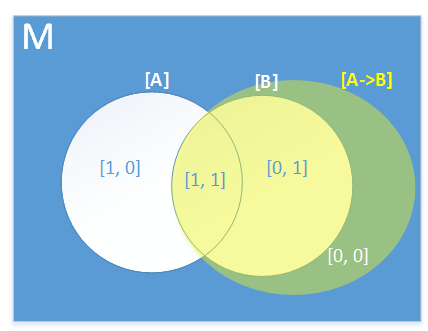
\includegraphics[width=0.75\textwidth]{images/A_implies_B.png}
\end{center}
\end{proof}

\subsection{$[A \iff B] = M$ iff $[A] = [B]$}

\begin{proof}
From the truth table of $A \iff B$ we can see that the only case where the propositional formula results in 1 (true) is when $v(A) = 0$, $v(B) = 0$ or $v(A) = 1$, $v(B) = 1$. Consequently, $[A \iff B] = \{[0, 0], [1, 1]\}$.
\begin{center}
    \begin{tabular}{c|c||c}
        \toprule
        A & B & $A \iff B$ \\ 
        \midrule
        0 & 0 & 1 \\
        0 & 1 & 0 \\
        1 & 0 & 0 \\ 
        1 & 1 & 1
    \end{tabular}
\end{center}

Intuitively, we can see that assignments $[0, 0] \subseteq  [A], [B]$ and $[1, 1] \subseteq [A], [B]$. In other words, in order to satisfy $[A \iff B]$, the valuations $[1, 0]$ and $[0, 1]$ have to be excluded from all the set of all possible valuations $M$, which yields $[A] = [B]$. This way the valuations in $[A \iff B]$ always result in a true assignment and ensure that the formula is a tautology.  A visual explanation of the proof is displayed below through a Venn-diagram. 
\begin{center}
	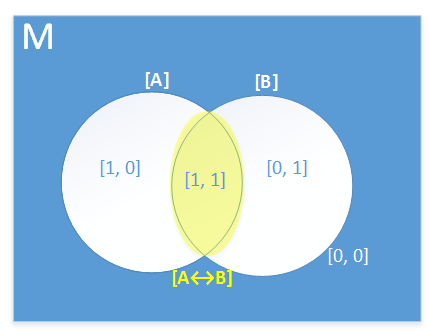
\includegraphics[width=0.75\textwidth]{images/A_iff_B.png}
\end{center}
\end{proof}


\section{Problem 5 - Exclusive disjunction (XOR, $\oplus$)}
\begin{center}
    \begin{tabular}{c|c||c}
        \toprule
        A & B & \boldmath{$A \oplus B$}  \\ 
        \midrule
        0 & 0 & 0 \\
        0 & 1 & 1 \\
        1 & 0 & 1 \\
        1 & 1 & 0
    \end{tabular}
\end{center}

\lastpage

\end{document}